\section{Model specifications and learning sensitivity}
\label{sec:model_details}
\begin{table}[pos=htbp]
\centering\small
\caption{Model families, their estimation and their role in the study.}
\label{tab:model_roles}
\renewcommand{\arraystretch}{1.13}
\begin{tabularx}{\linewidth}{@{}>{\raggedright\arraybackslash}p{0.19\linewidth}>{\raggedright\arraybackslash}p{0.27\linewidth}>{\raggedright\arraybackslash}X@{}}
\toprule
Model family & Behavioral specification & Estimation and role \\
\midrule
Joint neural Students & Shared representations with separate choice and departure outputs & Four objectives trained under matched conditions isolate the effect of the loss. Probability responses and timing are evaluated with separately selected fits. \\
MNL-S with separate timing & Linear choice utilities and an independently estimated timing predictor & Same inputs and training states, with a separately regularized choice model. Compares functional specifications and the separation of outcomes. \\
Supply-adapted Student & Adapted joint neural model with additional PT attributes & Differs in initialization, objective, auxiliary supervision and treatment of availability. Evaluated as an additional model, not as part of the matched loss comparison. \\
\bottomrule
\end{tabularx}
\end{table}
The neural model normalizes utilities over the available set $\mathcal A(\mathbf x)$:
\begin{equation}
p_{S,m}(\mathbf x)=\frac{\exp(u_m)}{\sum_{k\in\mathcal A(\mathbf x)}\exp(u_k)},\quad m\in\mathcal A(\mathbf x).
\label{eq:utility}
\end{equation}
Unavailable alternatives receive zero probability. MNL-S replaces the neural utilities with linear utilities on the same encoded information. Its coefficients are not constrained to have behavioral signs.
\subsection{Response-aware learning objectives}
\label{sec:loss_details}
Four objectives are compared within the joint architecture. With $H_1$ denoting the Huber loss with a one-minute transition, the objective at a single state is
\begin{equation}
\ell_{\mathrm{soft}}(\mathbf x)=D_{\mathrm{KL}}(\mathbf p_T\Vert\mathbf p_S)+H_1(\tau_S-\tau_T).
\label{eq:state}
\end{equation}
\emph{Soft KL} applies this loss to both states of every training pair. \emph{CE+KL} adds an equally weighted cross-entropy term for the Teacher's most likely mode, a hard label derived from its probability vector. The two response-aware objectives instead add a penalty on probability changes to soft KL and omit the hard label.

Within a training batch $\mathcal B$, let $a_{im}$ indicate that mode $m$ is available in at least one state of pair $i$. The \emph{signed-response} loss is
\begin{equation}
\ell_{\mathrm{signed}}=\frac{\sum_{i\in\mathcal B,m}a_{im}|\Delta p_{S,im}-\Delta p_{T,im}|}{\max(1,\sum_{i\in\mathcal B,m}a_{im})}.
\label{eq:signed}
\end{equation}
The \emph{direction+magnitude} objective penalizes the sign and the size of the response separately:
\begin{align}
\ell_{\mathrm{dir}}&=\frac{\sum_{i\in\mathcal B,m}a_{im}b_{im}[-\operatorname{sgn}(\Delta p_{T,im})\Delta p_{S,im}]_+}{\max(1,\sum_{i\in\mathcal B,m}a_{im}b_{im})},\label{eq:direction}\\
\ell_{\mathrm{mag}}&=\frac{\sum_{i\in\mathcal B,m}a_{im}\big||\Delta p_{T,im}|-|\Delta p_{S,im}|\big|}{\max(1,\sum_{i\in\mathcal B,m}a_{im})},\label{eq:magnitude}
\end{align}
where $b_{im}=\mathbf1(|\Delta p_{T,im}|>10^{-6})$ and $[u]_+=\max(u,0)$. Both terms carry unit weight. Their denominators differ because the direction term ignores negligible Teacher responses. The auxiliary supervision of SA-Student plays no part in this comparison.

Paired supervision changes the geometry of the fitting objective: it prioritizes differences between states whose endpoint targets are shared by all controlled models. Thus any improvement is attributable to response weighting under the matched protocol, not to additional Teacher information. Writing $\mathbf e(\mathbf x)=\mathbf p_S(\mathbf x)-\mathbf p_T(\mathbf x)$ for the endpoint error,
\begin{equation}
\|\Delta\mathbf p_S-\Delta\mathbf p_T\|_1\leq\|\mathbf e(\mathbf x')\|_1+\|\mathbf e(\mathbf x)\|_1,
\label{eq:bound}
\end{equation}
so a Student that matched the Teacher exactly at every state would also reproduce every response. The experiment tests response weighting under finite coverage and capacity. These penalties are optimization targets, not directional constraints: equally normalized direction and magnitude terms can have cancelling gradients on an interval of wrong-sign responses, and CE+KL changes the idealized single-state target. Appendix~\ref{sec:loss_diagnostics} derives both properties. The direct signed-response objective supplies a comparison that does not rely on splitting sign and magnitude.

\subsection{Properties of the learning objectives}
\label{sec:loss_diagnostics}
The signed and direction+magnitude objectives add response penalties to soft KL and place no weight on the hard-label cross-entropy, which only CE+KL includes. The persona, mechanism and accessibility supervision used to adapt SA-Student plays no part in the controlled comparison.

For a freely fitted state with common probability support and equal CE and KL weights,
\begin{equation}
\arg\min_{\mathbf p}\{\mathrm{CE}(a_T,\mathbf p)+D_{\mathrm{KL}}(\mathbf p_T\Vert\mathbf p)\}=\frac{\mathbf p_T+\mathrm{onehot}(a_T)}{2}.
\end{equation}
This optimum sharpens the Teacher distribution, and when the Teacher's leading mode is the same in both states of a pair, it halves the idealized probability difference. The fitted networks behave in the opposite way. On the 334 test pairs with an unchanged leading mode, the $L_1$ magnitudes of the responses, 0.1555, 0.1662 and 0.1876 under soft KL for the three seeds, rise to 0.1810, 0.1910 and 0.2280 under CE+KL. Parameter sharing and finite optimization thus shape the fitted response in ways the single-state solution does not predict.

For Teacher response $t>0$ and Student response $s\in[-t,0]$, equally normalized direction and magnitude terms satisfy
\begin{equation}
[-s]_+ + |t-|s||=t.
\end{equation}
The direction term is normalized by the number of available modes with a non-negligible Teacher response, and the magnitude term by the number of all available modes. The loss is flat over this interval whenever the two counts coincide, which holds for 357 of the 398 test pairs when each pair is evaluated alone, although the composition of a batch can change it. In a three-mode example with baseline $(0.4,0.3,0.3)$, a Teacher change of $(0.2,-0.1,-0.1)$ and a Student change of $(-0.1,0.05,0.05)$, the response gradients cancel while the endpoint losses remain active. A mode with a negligible Teacher response alters the normalization and removes the flat region. Figure~\ref{fig:loss_robustness} illustrates the loss surface and the sensitivity to individual personas.
\begin{figure}[pos=htbp]
\centering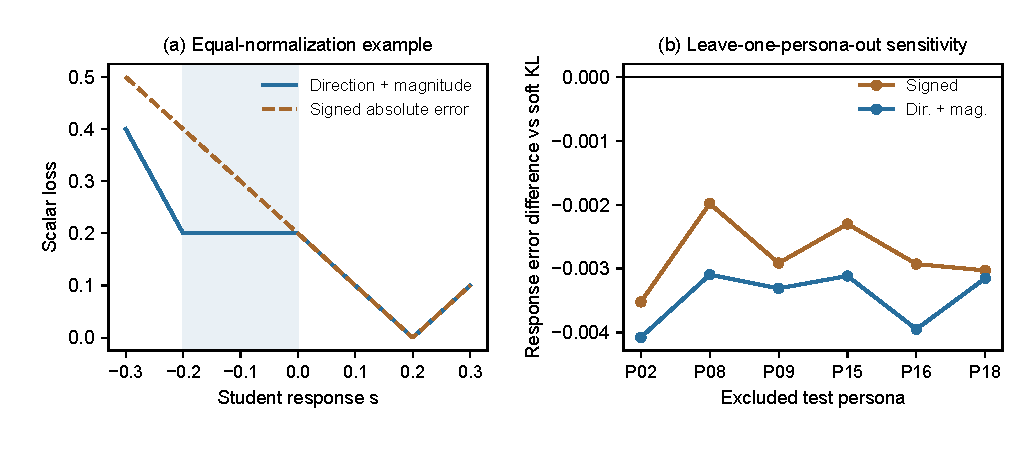
\includegraphics[width=.93\textwidth]{figures/revision20260921/figureS_revision_diagnostics.pdf}
\caption{Loss and persona sensitivity. Left: the equal-normalization direction+magnitude penalty and signed absolute error for a Teacher response of 0.2. Right: paired-objective response errors relative to soft KL after omitting each test persona from evaluation. Points average three fitted seeds; models are not retrained.}
\label{fig:loss_robustness}
\end{figure}


\subsection{Weight, selection and specification checks}
\label{sec:optimization_support}
The response-weight grid contains $\lambda\in\{0.25,0.5,1,2\}$ for signed-response and direction-plus-magnitude fitting, plus soft KL, each with three seeds. All 27 fits run for 120 epochs and 6,360 updates. Two validation selectors retain checkpoints from the same trajectory: macro-source KL and mean response error. Nine historical unit-weight configurations reproduce their parameters and selected epochs. The grid is a sensitivity analysis; the formal primary comparison retains unit-weight signed response and the KL selector.
\begin{figure}[pos=htbp]
\centering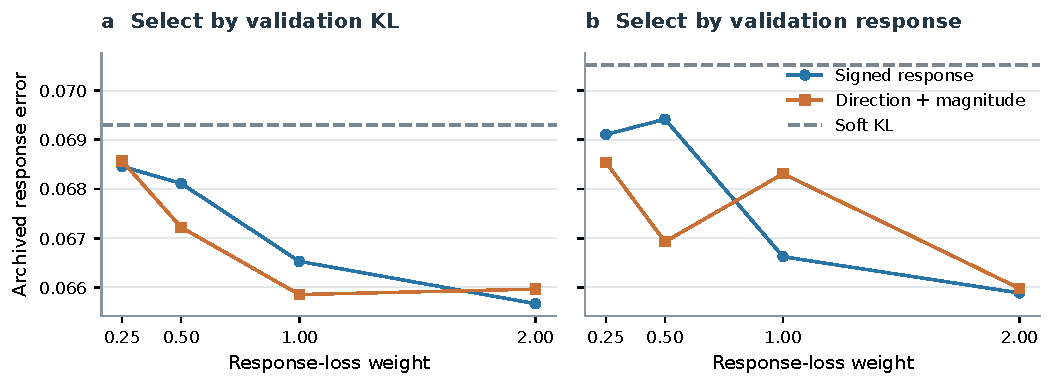
\includegraphics[width=\linewidth]{figures/revision20260925/figureA_weights.pdf}
\caption{Response-weight and validation-selector sensitivity on the archived benchmark. Points are means over three seeds on the same six test personas, not independent replications. Lines connect discrete fitted weights. Test minima are not used for post-hoc primary model selection.}
\label{fig:weight_sensitivity}
\end{figure}
The delay-withheld setting retains 1,562 training and 307 validation endpoints, after removing 277 and 58 respectively. Whole linked delay groups are removed, including zero-delay members. Its six fits use 120 epochs and 5,280 updates. On the 58 archived delay pairs, signed-response minus soft-KL error is $+0.00313$ ($[0.00182,0.00494]$) under KL selection and $+0.00532$ ($[0.00362,0.00715]$) under response selection. These retrospective intervals are conditional on only six personas. They agree in direction with the formal delayed-state result but are not an independent human test.

All four MNL regularization candidates converge; both choice selectors choose $10^{-4}$. A finite-perturbation diagnostic at the 39 explicitly feasible test endpoints increases fare by one unit, total PT time by five minutes, or access and total time jointly by five minutes. The latter two reduce PT probability at every endpoint; fare increases raise it at one third. These local directions do not identify willingness to pay or a value of travel time. Fixed-batch gradient records separate KL, departure and response terms along training; they are optimization diagnostics, not evidence of a causal mechanism for the loss advantage.

\subsection{Supply-adapted Student}
\label{sec:s9_recipe}
SA-Student adapts a previously trained joint neural Student to six additional PT-supply fields. The existing weights, categorical vocabularies and normalization are kept. The input weights for the new fields start at zero, and their normalization is fitted on the accessibility training states. The adapted model has 24,562 parameters. The accessibility supervision contains 336 states, divided into 234 for training, 51 for validation and 51 for testing, with disjoint pools of 79, 14 and 20 origin--destination pairs and of 28, six and six personas. Its targets average three Teacher queries for 89 states and five for 247, 1,502 valid queries in total.

\begin{table}[pos=htbp]
\centering\small
\caption{Specification and selection of the supply-adapted Student.}
\label{tab:s9_spec}
\renewcommand{\arraystretch}{1.14}
\begin{tabularx}{\linewidth}{@{}p{0.27\linewidth}X@{}}
\toprule
Item & SA-Student configuration \\
\midrule
Initialization & Previously trained joint Student; weights of the six added supply fields set to zero \\
Parameters & 24,562 \\
Accessibility split & 234 / 51 / 51 states (training / validation / test) \\
State-level objective & CE + KL for mode choice; Huber loss with one-minute transition for departure \\
Additional supervision & Direction/magnitude, mechanism, persona and accessibility contrasts \\
Supervision sources & Single-context : joint context : mechanism : accessibility = 2:1:1:1, with additional persona and accessibility-curve updates \\
Optimizer & Adam; learning rate $1.25\times10^{-4}$; weight decay $10^{-4}$ \\
Batch sizes & 32 states/pairs; eight mechanism quadruplets \\
Training schedule & Seed 42; maximum 120 epochs; patience 15 \\
Selection & Minimum KL on accessibility validation states, subject to at most a one-point loss in single-context accuracy and at most 10\% increases in single-context KL and in KL on joint contexts seen in training, relative to initialization \\
Selected epoch & 17 \\
Evaluation & Weights fixed in the stated-choice and simulation experiments \\
\bottomrule
\end{tabularx}
\end{table}

SA-Student applies the direction and magnitude terms of the main text to the modes available in the perturbed state, whereas the controlled comparison uses the modes available in either state. Mechanism supervision matches the responses from a baseline to variants that change the context together with the attributes, the context alone or the attributes alone. Persona supervision matches differences between travelers making the same trip, and accessibility supervision matches the PT response between the best and worst accessibility classes for a fixed traveler and trip.

Each epoch draws 104 single-context pairs and 52 each of joint-context pairs, persona pairs, accessibility states and accessibility-curve pairs, limited by the size of the available pools, while mechanism updates use the available groups of four states. All active loss terms have unit weight, and each type of update keeps its own reduction by sum or mean. The supplementary data files describe these settings and include the accessibility prompt. Because its initialization, additional supervision and adaptation differ from the controlled objectives of Section~\ref{supp-sec:supp_controlled}, SA-Student is not treated as part of the matched comparison of objectives. The predecessor checkpoint and its training history are retained in the corresponding model release.
\FloatBarrier

